\section{Architecture}
\begin{frame}{Architecture}
	\hspace{2.5cm} 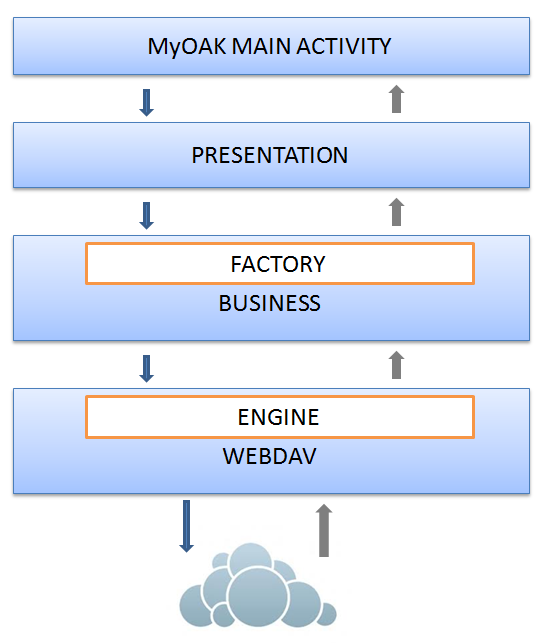
\includegraphics[scale=0.42]{img/Archi}
\end{frame}

\begin{frame}{WebDAV}
	\begin{itemize}
	\item \textbf{Web} \textbf{D}istributed \textbf{A}uthoring and \textbf{V}ersioning
	\item Extension du protocole HTTP
	\item But: Facilciter la gestion des fichiers avec des serveurs distants
		\begin{itemize}
		\item Récupérer
		\item Déposer
		\item Synchroniser
		\item Publier
		\item Accès concurrents
		\end{itemize}
	\end{itemize}
\end{frame}
		
\begin{frame}{Business}
	\begin{itemize}
		\item Couche métier
		\item Design pattern Composite
	\end{itemize}
	\hspace{3cm} 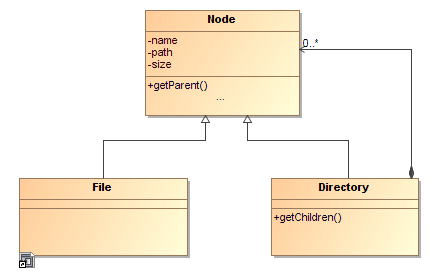
\includegraphics[scale=0.6]{img/designComposite}
\end{frame}		
		
\begin{frame}{Présentation}
	\begin{itemize}
		\item Séparation avec les modèles métiers
		\item Utilisation de la délégation
	\end{itemize}
	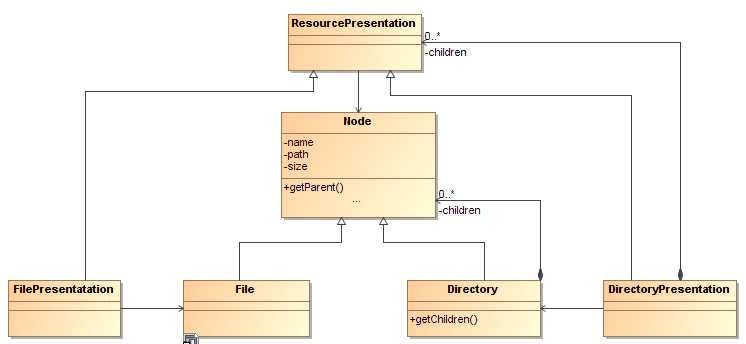
\includegraphics[scale=0.5]{img/presentation}
\end{frame}	

\begin{frame}{MyOAK Main Activity}
	\begin{itemize}
		\item Activité principale et unique de l’application
			\begin{itemize}
			\item Un fragment statique (Menu général)
			\item Un fragment dynamique
			\end{itemize}
		\item Un fragment pour chaque menu
		\item Chaque fragment ajoute ses options dans la barre d’action
	\end{itemize}
\end{frame}	
